\documentclass[11pt]{article}

\usepackage[margin=1in]{geometry}
\usepackage{amsmath,amssymb}
\usepackage[dvipsnames]{xcolor}
\usepackage{hyperref}
\usepackage{microtype}
\usepackage{graphicx}

\setlength{\parindent}{0pt}
\setlength{\parskip}{1em}

% Remove footnote indentation
\usepackage[hang,flushmargin]{footmisc}

\hypersetup{
    colorlinks=true,
    linkcolor=green!40!black,
    citecolor=green!40!black,
    urlcolor=green!40!black
}

\title{\Large\bf Hume's Representational Conditions for Causal Judgment:\\ What Bayesian Formalization Abstracted Away}

\author{Yiling Wu\\
\normalsize BridgeM, Inc.\\
\normalsize Department of Philosophy, University of Massachusetts Amherst}

\date{}

\begin{document}

\maketitle
\thispagestyle{empty}

\begin{abstract}
\noindent Hume's account of causal judgment presupposes three representational conditions: experiential grounding (ideas must trace to impressions), structured retrieval (association must operate through organized networks exceeding pairwise connection), and vivacity transfer (inference must produce felt conviction, not merely updated probability). This paper extracts these conditions from Hume's texts and argues that they are integral to his causal psychology. It then traces their fate through the formalization trajectory from Hume to Bayesian epistemology and predictive processing, showing that later frameworks preserve the updating structure of Hume's insight while abstracting away these further representational conditions. Large language models serve as an illustrative contemporary case: they exhibit a form of statistical updating without satisfying the three conditions, thereby making visible requirements that were previously background assumptions in Hume's framework.

\vspace{0.5em}
\noindent \emph{Keywords: Hume, causal judgment, Bayesian epistemology, predictive processing, representational conditions, formalization, representational structure}
\end{abstract}

\section{Introduction}

Hume's account of causal inference describes a process in which the mind, having repeatedly observed the conjunction of two types of events, forms a habit of expecting the second upon the appearance of the first. This habit produces a distinctive felt transition, an impression of determination, which Hume identifies as the source of our idea of necessary connection.\footnote{Hume, \emph{Treatise} 1.3.14.1 (SBN 155-6); \emph{Enquiry} 7.2.28-9 (SBN 75-6). All references to the \emph{Treatise} follow the Norton and Norton edition (Oxford, 2000); references to the \emph{Enquiry} follow the Beauchamp edition (Oxford, 2000). I use the standard abbreviated forms: T for the \emph{Treatise}, E or EHU for the \emph{Enquiry}.} The structure of this process is widely recognized as anticipating Bayesian conditionalization, in which evidence modifies prior belief to yield posterior belief according to a principled updating rule.\footnote{Earman, \emph{Bayes or Bust?}, ch. 1. The structural parallel between Humean custom and Bayesian conditionalization has been noted by many commentators, though, as Earman observes, the application of Bayesian formalism to Hume is strictly anachronistic: Bayes' theorem is not to be found in Hume's writings.} Predictive processing extends this inheritance computationally.\footnote{Clark, \emph{Surfing Uncertainty}; Hohwy, \emph{The Predictive Mind}; Friston, ``The Free-Energy Principle.''}

This paper argues that the trajectory, while preserving the updating structure that constitutes Hume's central insight, has at each step abstracted away a set of representational conditions that Hume's original theory required. Three conditions are identified. The first, experiential grounding, requires that the ideas involved in causal inference trace back to impressions derived from sensory experience. The second, structured retrieval, requires that association operate within an organized system of ideas, including what Don Garrett has called the revival set, rather than through arbitrary co-occurrence. The third, vivacity transfer, requires that the inferential transition produce a qualitative change in the status of the activated idea, transforming it from mere thought into belief through the transmission of force and vivacity from a present impression. Each of these conditions is integral to Hume's explanation of how the mind moves from observed conjunction to causal judgment, and each has been progressively abstracted away in the formalization from Hume to Bayes to predictive processing.

A methodological note is needed at the outset. The three representational conditions identified in this paper have each been individually recognized in various strands of Hume scholarship, but they have not been systematically extracted as a group or traced through the formalization trajectory that connects Hume to contemporary Bayesian cognitive science. The paper's primary contribution is this extraction and tracing. Large language models appear only as an illustrative case in the final section: they make the abstracted conditions visible by exhibiting a system that instantiates the updating structure without satisfying any of the three conditions, but the interpretive thesis about Hume does not depend on any particular empirical claim about LLM capabilities.

The paper proceeds as follows. Section 2 analyzes Hume's representational architecture, focusing on the copy principle, the memory/imagination distinction, and the revival set mechanism. Section 3 extracts the three representational conditions from Hume's account of causal inference and causal judgment. Section 4 traces the formalization path from Hume through Bayesian epistemology to predictive processing and identifies what each step preserved and what it abstracted away. Section 5 briefly illustrates the abstracted conditions through the case of large language models. Section 6 concludes.

\section{Hume's Representational Architecture}

\subsection{Impressions, Ideas, and the Grounding Condition}

Hume's theory of mind begins with a distinction between two kinds of perception: impressions and ideas. Impressions are the original perceptions of the mind, arising from sensation or reflection, and are characterized by their force and vivacity. Ideas are fainter copies of impressions, derived from them and dependent on them for their content.\footnote{T 1.1.1.1 (SBN 1-2). Hume initially distinguishes impressions and ideas in terms of their relative force and vivacity, though he was never fully satisfied with this characterization. See Garrett, \emph{Hume}, ch. 2, for a careful discussion of the difficulties.} The Copy Principle establishes the dependency: every simple idea is a copy of a corresponding simple impression, and the mind's creative power consists solely in compounding, transposing, augmenting, or diminishing the materials that sensation and experience provide.\footnote{T 1.1.1.7 (SBN 4); EHU 2.5 (SBN 19). Hume allows a famous exception: the missing shade of blue (T 1.1.1.10, SBN 5-6). The exception is widely discussed but does not undermine the general principle. See Garrett, \emph{Cognition and Commitment}, ch. 2.}

The Copy Principle is typically read as a thesis about the origin of mental content: it tells us where our ideas come from. But it is also, and for present purposes more importantly, a grounding condition. It constrains what can serve as genuine content in the mind's operations. An idea that cannot be traced back to a corresponding impression is, for Hume, empty or confused. The point is vivid in Hume's discussion of the person born blind, who cannot form the idea of color, or the person born deaf, who cannot conceive of sound.\footnote{EHU 2.7 (SBN 20). Hume uses these cases to illustrate that without the relevant sensory impression, the corresponding idea simply cannot be formed.} Content, on this view, is not free-floating; it is anchored in perceptual experience.

This grounding condition will prove important when we turn to the Bayesian formalization of Hume's insight. In Bayesian epistemology, the hypothesis space over which updating occurs can be specified arbitrarily. There is no requirement that the hypotheses correspond to experientially grounded ideas. A Bayesian agent can have a prior over hypotheses it has never perceived and could never perceive. Hume's system does not allow this: ideas that lack an experiential basis are not eligible participants in the inferential machinery of custom and habit.\footnote{Fodor, \emph{Hume Variations}, ch. 1, emphasizes this point in connecting Hume's concept empiricism to contemporary debates about the origin of concepts. Landy, \emph{Hume's Science of Human Nature}, ch. 1, provides a detailed analysis of how the Copy Principle functions as a constraint on the cognitive system rather than merely a genetic thesis.}

\subsection{Memory, Imagination, and Operational Structure}

Hume distinguishes memory, which reproduces ideas in their original order, from imagination, which can freely rearrange and recombine them (T 1.1.3.1-3, SBN 8-10). This distinction establishes that Hume's representational space supports multiple modes of access and manipulation and therefore cannot be a flat collection of pairwise associations.\footnote{Garrett, \emph{Cognition and Commitment}, ch. 1; Owen, \emph{Hume's Reason}, ch. 6; Waxman, \emph{Hume's Theory of Consciousness}, ch. 3.} This architectural requirement is a precondition for the structured retrieval condition (RC-2) that Section 3 will extract; the revival set mechanism, to which we now turn, is the specific structure that satisfies it.

\subsection{Abstract Ideas, the Revival Set, and Prior Structure}

Hume holds that ideas are, in themselves, always particular: the idea of a triangle in the mind always has a specific shape, size, and proportion.\footnote{T 1.1.7.6 (SBN 19-20).} Generality arises not from any indeterminacy in the idea itself but from the mind's manner of using ideas. Two levels of commitment must be distinguished here. At the minimal textual level, Hume's own text establishes that when a particular idea is attached to a general term, the mind becomes disposed to ``raise up'' other particular ideas as needed: ``when we have found a resemblance among several objects \ldots\ we apply the same name to all of them'' and ``after we have acquired a custom of this kind, the hearing of that name revives the idea of one of these objects'' along with a readiness to summon others (T 1.1.7.7, SBN 20). This readiness to summon relevantly similar ideas in response to a general term is Hume's own claim, not a reconstruction imposed from outside. At the level of strong explanatory reconstruction, Garrett has developed this into a detailed account of what he calls the revival set: a dispositional set of ideas associated with a given exemplar, available for activation on demand for purposes of comparison and evaluation.\footnote{Garrett, \emph{Cognition and Commitment}, ch. 3, develops the revival set reading in full. See also Garrett, ``Hume's Theory of Ideas,'' in \emph{A Companion to Hume}. For objections, see Broughton, ``Explaining General Ideas''; for an alternative account, see Flage, ``Hume's Relative Ideas.''} The analysis that follows draws on Garrett's terminology for expository convenience, but the structural claims it makes require only the minimal textual commitment, not the full explanatory reconstruction.

The revival set mechanism works as follows. When the abstract idea of ``triangle'' is activated through its exemplar (say, a red equilateral triangle), and a judgment is made such as ``all triangles are equilateral,'' the mind's disposition to summon other ideas from the revival set is triggered: ideas of right-angled triangles and obtuse-angled triangles arise to refute the claim.\footnote{T 1.1.7.7-8 (SBN 20-1). Garrett's reading has been influential but not uncontested. Broughton, ``Explaining General Ideas,'' raises important objections concerning the mechanism by which the revival set is activated. These objections bear primarily on the psychological details of the activation process rather than on the structural point at issue here: that Hume's system requires a structured network of idea-connections that goes beyond pairwise association.} What matters for present purposes is the structural implication: ideas in Hume's system are not isolated atoms linked only by pairwise associations. They are organized into networks in which activation of one idea can trigger the retrieval of related ideas according to principles of resemblance, contiguity, and cause and effect.\footnote{Flage, ``Hume's Relative Ideas,'' discusses how Hume's ideas stand in complex relational structures that cannot be reduced to simple copies of impressions.}

This revival set structure is, in functional terms, Hume's version of a prior knowledge structure. When a new impression arrives, the revival set determines which related ideas are available for retrieval, comparison, and judgment. The functional parallel to the Bayesian prior is clear: both specify what background knowledge the system brings to bear on new evidence. But Hume's version has two features that the Bayesian prior lacks. First, the contents of the revival set are experientially grounded: they consist of ideas derived from impressions, not arbitrary mathematical objects. Second, the connections among ideas in the revival set are established through actual experience and the principles of association, not through stipulation.\footnote{Fodor, \emph{Hume Variations}, ch. 4, connects Hume's theory of abstract ideas to contemporary debates about concept structure and argues that Hume's account is more sophisticated than is typically appreciated.}

A further structural feature emerges from this analysis. Hume's cognitive architecture operates on two distinct layers (see Figure 1).

\begin{figure}[ht]
\centering
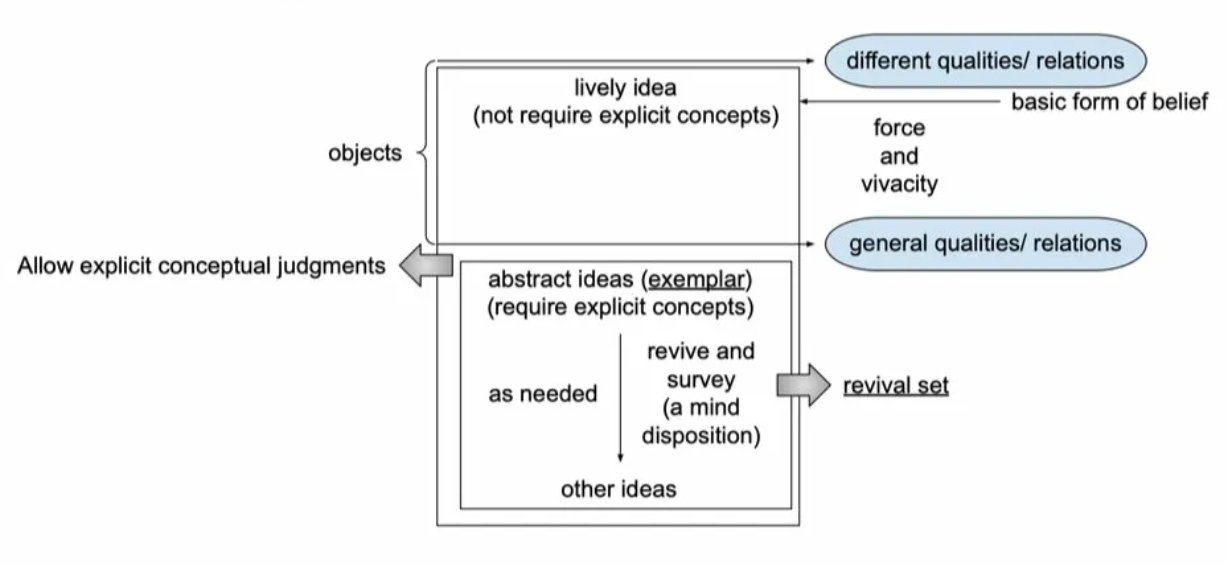
\includegraphics[width=0.75\textwidth]{fig3.png}
\caption{Hume's dual-layer model of mental representation, illustrating the distinction between inference-level processing (lively ideas, force and vivacity, basic belief) and judgment-level processing (abstract ideas, exemplars, revival sets) that underwrites the extraction of RC-2.}
\label{fig:dual-layer}
\end{figure}

At the first layer, objects produce lively ideas through force and vivacity; these lively ideas constitute the basic form of belief and do not require the deployment of explicit concepts. A child who recoils from a flame operates at this layer. At the second layer, abstract ideas (exemplars) are associated with general terms and connected to revival sets, enabling explicit conceptual judgments about general qualities and relations. A scientist who judges that ``fire causes combustion'' operates at this layer. The two layers are not independent: the second layer is built on the first, because abstract ideas are themselves constructed from particular ideas that were originally copies of impressions. But they are functionally distinct, and the operations available at the second layer (summoning counterexamples, testing general propositions, applying concepts to new instances) are not available at the first.\footnote{This dual-layer reading is consistent with Garrett's analysis of the distinction between causal inference and causal judgment; see Garrett, ``Hume on Causation,'' pp. 77-9. Landy, \emph{Hume's Science of Human Nature}, ch. 3, provides a contemporary cognitive-scientific framework for understanding the layered structure of Hume's representational system.}

It is worth pausing to address a significant objection to the revival set reading. Broughton has argued that Garrett's account of how the revival set is activated faces a circularity: the mechanism that is supposed to summon relevant ideas from the revival set seems to require that the mind already know which ideas are relevant, which presupposes the very general knowledge that the revival set is meant to explain.\footnote{Broughton, ``Explaining General Ideas,'' pp. 283-7.} This objection is important, but it bears primarily on the psychological details of the activation mechanism rather than on the structural point at issue in this paper. Even if the precise mechanism of revival set activation remains an open question, the structural requirement is clear: Hume's system needs something that goes beyond pairwise association. The mind's ability to summon diverse particular ideas in response to a general term, and to use those ideas to evaluate general propositions, requires an organized network of connections among ideas. It is this structural requirement, not the specific mechanism by which it is implemented, that is abstracted away in the Bayesian formalization.

The three components analyzed in this section, the grounding of ideas in impressions, the operational structure of memory and imagination, and the organized retrieval system of the revival set, are not offered here as a survey of Hume's philosophy of mind. They are the evidential basis from which the next section will extract three minimum representational conditions that Hume's account of causal judgment requires.

\section{The Representational Conditions of Causal Judgment}

A terminological clarification is needed before proceeding. This paper's target is causal judgment in the specific Humean sense: the explicitly conceptualized attribution of a causal relation between general kinds, as when we judge that ``fire causes burning.'' This is distinct from causal inference, which is the pre-conceptual transition from a present impression to a lively idea of the expected effect, and from the broader notion of causal cognition, which includes animal learning, infant prediction, and simple intervention competence. The three representational conditions extracted below are conditions on causal judgment so defined. They are not intended as conditions on all forms of causal cognition; systems that lack them may still exhibit causal inference in the pre-conceptual sense.

\subsection{Causal Inference: Custom, Vivacity, and Belief}

Hume's account of causal inference can be decomposed into a sequence of steps. The mind observes the constant conjunction of two types of events. Through repetition, custom or habit produces a propensity to expect the second event upon the appearance of the first. When a present impression of the first event occurs, this propensity causes the mind to form an idea of the second event. The associative transition transmits force and vivacity from the present impression to the associated idea, enlivening it beyond the degree characteristic of mere imagination. This enlivened idea constitutes belief.\footnote{T 1.3.7.5 (SBN 96-7); EHU 5.1.5-12 (SBN 43-8). Owen, \emph{Hume's Reason}, ch. 6, provides a detailed reconstruction of this inferential process.}

The process can be represented schematically (see Figure 2). A present impression of object A, connected through custom to the idea of object B, produces a transition in which force and vivacity flow from the impression to the idea, generating belief in B's occurrence. The impression of determination, which is an impression of reflection (internal), accompanies this transition and constitutes the origin of our idea of necessary connection.\footnote{T 1.3.14.1 (SBN 155-6). Garrett, ``Hume on Causation,'' pp. 73-88, develops the ``causal sense'' interpretation: the entire mechanism, from constant conjunction through associative inference to the impression of necessary connection, constitutes a causal sense analogous to Hume's moral sense and aesthetic sense.}

\begin{figure}[ht]
\centering
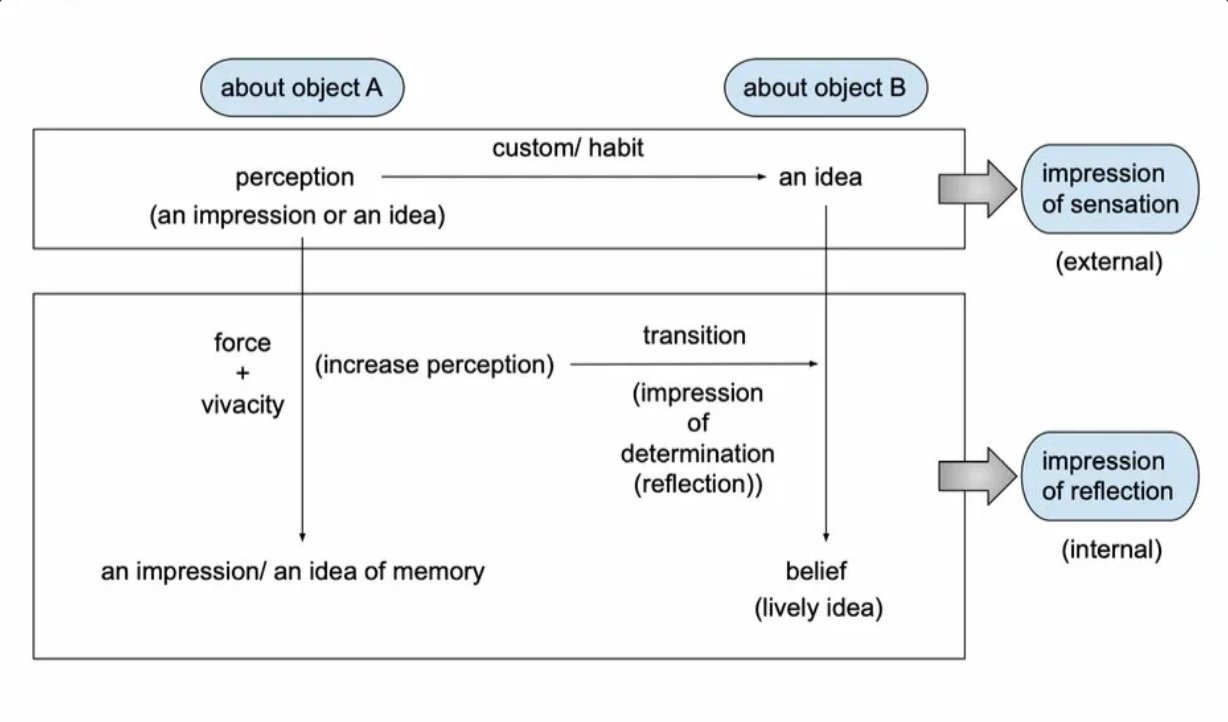
\includegraphics[width=0.85\textwidth]{fig1.png}
\caption{Hume's account of causal inference, showing the pathway from perception through custom/habit to belief (lively idea). The impression of determination (an impression of reflection) accompanies this transition and provides the experiential basis for RC-3 (vivacity transfer).}
\label{fig:causal-inference}
\end{figure}

Three representational conditions are implicit in this process.

\emph{RC-1 (Experiential Grounding).} The ideas involved in causal inference must trace back to impressions. The content of the cause-idea and the effect-idea must be derived from actual sensory experience, not from symbolic association or arbitrary stipulation. Without this grounding, the ideas lack the content that makes the associative transition genuinely about the events in question. Hume is explicit that the mind's creative power is limited to compounding, transposing, augmenting, and diminishing the materials furnished by the senses and experience (EHU 2.5, SBN 19). When we form the causal judgment that fire causes burning, the ideas of fire and burning must each originate in actual perceptual encounters with fire and burning. An agent that has never had the relevant impressions cannot form these ideas and therefore cannot undergo the causal inference that connects them. The Copy Principle is not merely a genetic thesis about the origin of ideas; it is a constraint on what can serve as input to the machinery of custom and belief.\footnote{Garrett, \emph{Cognition and Commitment}, ch. 2, argues that the Copy Principle functions as a methodological tool in Hume's philosophy, not merely a psychological generalization. Landy, \emph{Hume's Science of Human Nature}, ch. 1, develops this point in detail, showing how the Copy Principle constrains the cognitive system's operations rather than merely describing its history.}

\emph{RC-2 (Structured Retrieval).} The association between the cause-idea and the effect-idea must operate within an organized system of ideas, not through arbitrary co-occurrence. The textual basis for this condition does not depend on any single commentator's reconstruction. Hume's own account of abstract ideas requires it. When we use a general term like ``fire,'' the mind must be able to recognize a particular perception as an instance of the general kind, and must be disposed to summon other instances of the kind when a general proposition is asserted or challenged (T 1.1.7.7-8, SBN 20-1). Hume is explicit that a particular idea, when attached to a general term, ``raises up'' other particular ideas as needed (T 1.1.7.7, SBN 20). This raising-up operation requires more than pairwise association between two specific ideas; it requires an organized set of ideas connected by resemblance that can be activated on demand. This much is a textual claim about Hume's theory, not a reconstruction imposed from outside.

The strongest explanatory model of how this organized set functions is Garrett's revival set reading, according to which a particular idea serving as exemplar is associated with a dispositional readiness to summon relevantly similar ideas for comparison and evaluation.\footnote{Garrett, \emph{Cognition and Commitment}, ch. 3, develops the revival set reading in full. Garrett, ``Hume's Theory of Ideas,'' provides a condensed version. For objections, see Broughton, ``Explaining General Ideas''; for an alternative account of relational structure among Hume's ideas, see Flage, ``Hume's Relative Ideas.''} But the structural requirement that RC-2 names does not stand or fall with Garrett's specific account of the activation mechanism. It stands on Hume's own text: if abstract ideas require organized retrieval of relevantly similar ideas, and if causal judgment requires abstract ideas (to classify particular instances under general kinds like ``cause'' and ``effect''), then causal judgment requires organized retrieval. Any interpretation of Hume that accepts these two premises must accept RC-2, whatever mechanism it attributes to the retrieval process.

Causal judgment places a distinctive demand on this retrieval structure. Unlike purely classificatory judgment (``this is a triangle''), causal judgment requires connecting two distinct general kinds across a temporal and experiential gap, and doing so defeasibly across novel instances. Judging that fire causes burning requires simultaneously deploying the conceptual resources associated with ``fire'' and ``burning,'' recognizing the causal relation as holding generally, and being disposed to survey counterexamples.\footnote{Garrett, ``Hume on Causation,'' pp. 77-9, emphasizes that causal judgment requires the deployment of both definitions of ``cause'' simultaneously.} RC-2 is therefore a condition on what Hume's causal judgment requires of the representational system, not a thesis about how one particular commentator reconstructs its psychology.

\emph{RC-3 (Vivacity Transfer).} The inferential transition must produce a qualitative change in the status of the activated idea: it must be transformed from mere thought into belief through the transmission of force and vivacity from a present impression. This is not simply a matter of assigning a higher probability; it is the production of a felt quality that makes the idea function as if it were a perception rather than a fantasy. Hume insists that belief is ``a lively idea related to or associated with a present impression'' (T 1.3.7.5, SBN 96), and the liveliness is essential to its functional role. As Hume explains the mechanism: ``when any impression becomes present to us, it not only transports the mind to such ideas as are related to it, but likewise communicates to them a share of its force and vivacity'' (T 1.3.8.2, SBN 98). The result is that the idea of the effect, when activated through the causal transition, is not merely entertained as a possibility but felt as a conviction. This felt conviction is what Hume calls belief, and it is what distinguishes the causal expectation of a scientist from the idle fantasy of a daydreamer. The point is not merely phenomenological. Vivacity serves a functional role that cannot be replaced by a probability value: it is what makes the idea of the expected effect guide action, orient attention, and resist displacement by competing ideas. An idea conceived with vivacity produces behavioral readiness; the same idea conceived without vivacity does not. For Hume, the difference between believing that fire will burn and merely entertaining the proposition that fire will burn is not a difference in content but a difference in the manner of conception (T 1.3.7.7, SBN 97), and this difference in manner is what enables belief to function as a practical guide. RC-3 is therefore not a phenomenological ornament attached to an otherwise functional account; it names the mechanism by which Hume's system transitions from cognitive processing to action-guiding conviction.\footnote{Loeb, \emph{Stability and Justification in Hume's Treatise}, ch. 3, discusses the role of stability in Hume's theory of belief and argues that vivacity alone is insufficient; stability, produced by custom, is also required. Everson, ``The Difference between Feeling and Thinking,'' provides a careful analysis of the force/vivacity distinction. Miyazono, ``Hume and the Cognitive Phenomenology of Belief,'' argues that Hume's belief has a distinctively cognitive phenomenology that is different in kind from sensory force and vivacity, further supporting the claim that vivacity transfer is not reducible to a numerical change in probability.}

The impression of determination, which accompanies the causal transition, is particularly important for understanding RC-3. It is an impression of reflection (internal), not an impression of sensation (external). That is, it arises from the mind's awareness of its own inferential transition, not from the observation of any external connection between events (see Figure 3). Hume's analysis thus requires a system that can distinguish between external perceptions and internal reflective states, and that can generate the latter as a product of its own inferential operations. This capacity for reflective self-awareness has no analogue in Bayesian updating, which produces revised probability values without any corresponding internal phenomenology.\footnote{Garrett, ``Hume on Causation,'' pp. 85-8, develops the ``causal sense'' interpretation in detail, arguing that the impression of determination functions analogously to a sensory impression: it provides the experiential basis for our idea of necessary connection, just as sensory impressions provide the experiential basis for our ideas of color, sound, and shape.}

\begin{figure}[ht]
\centering
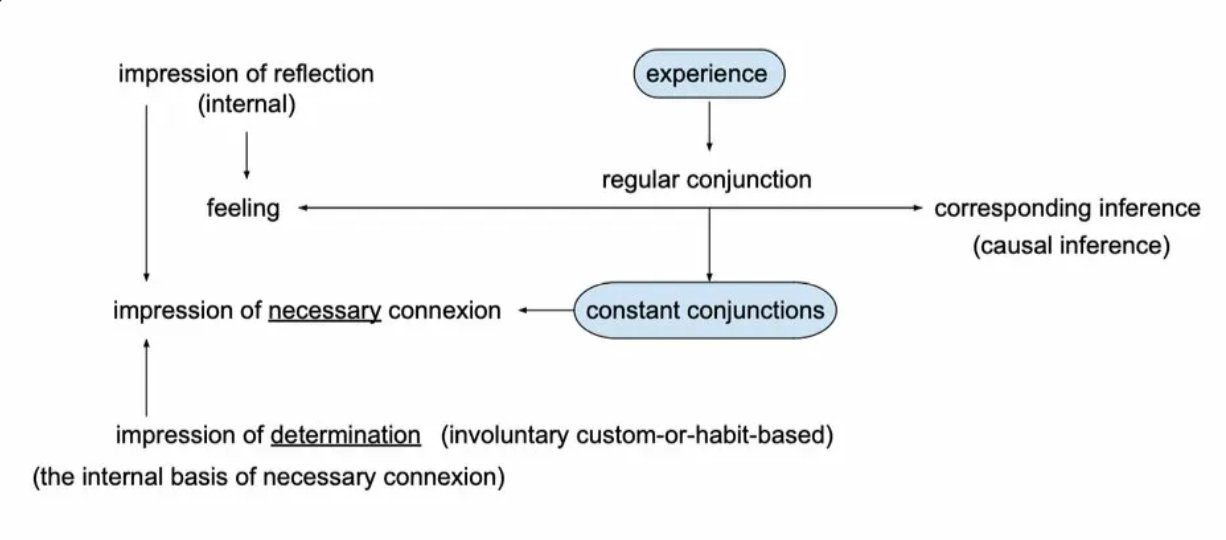
\includegraphics[width=0.75\textwidth]{fig2.png}
\caption{Hume's model of how the idea of necessary connection arises. The impression of determination is internal (an impression of reflection), not derived from external observation, illustrating why RC-3 requires a system capable of distinguishing external perceptions from internal reflective states.}
\label{fig:necessary-connection}
\end{figure}

\subsection{Causal Judgment: The Revival Set in Causal Cognition}

A distinction must be drawn between causal inference and causal judgment. Causal inference, as described in Section 3.1, is a pre-conceptual process: it produces a lively idea (belief) without requiring the deployment of explicit concepts. A dog that expects food upon hearing a bell undergoes causal inference. Causal judgment, by contrast, is an explicitly conceptualized judgment of the form ``Object A and Object B are cause and effect.''\footnote{Garrett, ``Hume on Causation,'' p. 77, draws this distinction and argues that Hume's two definitions of ``cause'' correspond to these two levels: the first definition (constant conjunction) describes the experiential basis of causal inference, while the second definition (association-plus-inference) describes the mental process involved in causal judgment.}

This distinction maps onto the dual-layer structure of Hume's representational architecture identified in Section 2.3. At the first layer, objects produce lively ideas through force and vivacity; this is the level of causal inference, where belief arises without explicit conceptual structure. At the second layer, abstract ideas are deployed through the revival set mechanism; this is the level of causal judgment, where the mind classifies particular instances under general kinds and applies causal concepts. Hume's two definitions of ``cause'' correspond precisely to these two layers. The first definition characterizes cause at the experience level (external): ``An object precedent and contiguous to another, and where all the objects resembling the former are placed in like relations of precedency and contiguity to those objects that resemble the latter'' (T 1.3.14.31, SBN 170). The second definition characterizes cause at the mental determination level (internal): ``A cause is an object precedent and contiguous to another, and so united with it that the idea of the one determines the mind to form the idea of the other, and the impression of the one to form a more lively idea of the other'' (T 1.3.14.31, SBN 170).\footnote{The relationship between Hume's two definitions has been extensively debated. Garrett, \emph{Cognition and Commitment}, ch. 5, argues that they are complementary rather than competing, each capturing a different aspect of the same phenomenon. Beebee, \emph{Hume on Causation}, ch. 3, provides an alternative analysis that emphasizes the tension between the definitions. For present purposes, the key point is that the second definition explicitly invokes mental determination, that is, the representational process by which the mind transitions from one idea to another.}

Causal judgment requires something that causal inference does not: the deployment of abstract ideas and the kind of organized retrieval structure that Garrett models as the revival set. To judge that fire causes burning is not merely to expect burning upon perceiving fire; it is to classify the particular instance under a general kind (``fire,'' ``burning'') and to apply a general causal principle. This requires organized retrieval: the exemplar idea of fire must be connected to a set of related ideas that can be summoned to support, test, or refine the judgment. When a particular instance of fire is perceived, the mind must be able to recognize it as an instance of the general kind ``fire,'' retrieve associated effects (burning, heat, light), and form the general judgment that fire causes these effects. This operation is categorically richer than the mere expectation that constitutes causal inference.\footnote{Garrett, \emph{Cognition and Commitment}, ch. 3, provides the fullest account of how this organized retrieval functions in Hume's theory of abstract ideas and their role in judgment.}

The distinction matters for the Bayesian formalization because Bayesian conditionalization models only the inference level. It captures how belief strength is updated in light of evidence. It does not capture the judgment level: the categorical structure required to classify particular instances under general kinds, to summon counterexamples from a revival set, or to apply general rules to particular cases. This categorical machinery is absent from Bayesian formalism, even though it is integral to Hume's account of how we form and deploy causal concepts.\footnote{Beebee, \emph{Hume on Causation}, ch. 3, discusses the relationship between Hume's two definitions of cause and argues that both are essential to his account. The inference/judgment distinction developed here aligns with Beebee's analysis while drawing out the representational implications.}

\subsection{General Rules and Self-Calibration}

This subsection only reinforces the claim that Humean causal judgment exceeds any purely first-order updating model; it does not expand the paper's main taxonomy. Hume recognizes that unchecked association produces erroneous judgments (T 1.3.13.7-12, SBN 146-50) and introduces general rules as higher-order principles by which the mind calibrates its own associative tendencies.\footnote{Hearn, ``General Rules in Hume's \emph{Treatise}''; Lyons, ``General Rules and the Justification of Probable Belief''; Kail, \emph{Projection and Realism in Hume's Philosophy}, ch. 4.} This meta-level capacity requires representational self-access that no purely first-order updating model provides, further supporting the claim that the three conditions identified above are integral to a system structurally richer than bare association.

\subsection{Interpretation-Neutrality of the Three Conditions}

A natural concern about the foregoing analysis is that it might depend on a particular interpretation of Hume's theory of causation. The literature on Hume's causation is divided among several major readings: the regularity (or reductionist) reading, according to which causation just is constant conjunction;\footnote{The regularity reading has its classic expression in the logical positivist tradition. Beebee, \emph{Hume on Causation}, ch. 2, provides a careful contemporary reconstruction.} the projectivist reading, according to which the mind projects an internally generated impression of necessity onto the external world;\footnote{The projectivist reading is developed by Blackburn, ``Hume and Thick Connexions,'' and others. Kail, \emph{Projection and Realism in Hume's Philosophy}, ch. 2, provides the most detailed analysis.} and the quasi-realist or skeptical realist reading, according to which Hume is agnostic about whether objective necessary connections exist but holds that we cannot know them if they do.\footnote{Strawson, \emph{The Secret Connexion}, argues for a realist reading according to which Hume believes in objective causal powers but holds that we cannot perceive them. Kail, \emph{Projection and Realism}, ch. 5, develops a more nuanced quasi-realist position. Millican, ``Hume, Causal Realism, and Causal Science,'' provides a comprehensive overview of the interpretive landscape.}

The three representational conditions identified in this paper are neutral among these interpretations. They are conditions on Hume's causal psychology, not on his causal metaphysics. Regardless of whether causation in the world is mere regularity, a projection of the mind, or an unknowable objective relation, the psychological process by which the mind arrives at causal beliefs requires experientially grounded ideas (RC-1), structured retrieval through associative pathways (RC-2), and vivacity transfer from impression to idea (RC-3). The regularity theorist, the projectivist, and the realist all agree on the psychological mechanism; they disagree about what, if anything, in the external world corresponds to the output of that mechanism. The three RCs are conditions on the mechanism, not on its correspondence to external reality. This interpretation-neutrality strengthens the paper's argument, because it means that the conditions identified here are not artifacts of a partisan reading of Hume but structural features of his causal psychology that any adequate interpretation must accommodate.

This concludes the paper's primary contribution: the systematic extraction of three representational conditions from Hume's causal psychology. The claim is that Hume's account of causal judgment cannot operate without experientially grounded ideas (RC-1), organized retrieval structures that exceed pairwise association (RC-2), and a mechanism for transmitting felt conviction from impression to idea (RC-3). The remaining sections trace what happened to these conditions in the intellectual trajectory that descends from Hume, and identify a contemporary system that makes their absence diagnostically visible. These subsequent sections depend on the interpretive thesis established here, but the thesis itself does not depend on them.

\section{From Hume to Bayes: What Was Preserved and What Was Abstracted Away}

The trajectory from Hume to Bayes to predictive processing crosses three distinct levels of theorizing: Hume's is a psychological-explanatory theory that describes actual mental operations; Bayesian epistemology is a normative-formal schema that specifies how a rational agent ought to update beliefs; predictive processing is a computational re-embedding that implements approximate Bayesian updating in a mechanistic architecture. The three levels are not interchangeable, and comparing them requires care. A methodological clarification is therefore in order. This section does not claim that Bayesian epistemology failed to preserve something it aimed to preserve; a normative-formal schema is not in the business of encoding psychological implementation details, and it would be a category mistake to fault it for not doing so. The claim is different: that the intellectual trajectory from Hume to Bayes to predictive processing constitutes a chain of explanatory inheritance under progressive formal abstraction, and that tracking what is preserved and what is abstracted away at each step is a legitimate and informative philosophical exercise. What makes the comparison legitimate is not that the three levels share a common subject matter but that each level inherits and transforms the updating insight of its predecessor. The question driving this section is: which features of Hume's original theory survive each transformation, and which do not?

\subsection{The Bayesian Formalization of Humean Updating}

The structural parallel between Hume's custom and Bayesian conditionalization can be stated precisely. Hume: repeated conjunction of events of type A and type B produces, through custom, a habit of expecting B upon observing A; the strength of this expectation is proportional to the uniformity and frequency of the observed conjunction. Bayes: the posterior probability P(H$|$E) is proportional to the prior probability P(H) multiplied by the likelihood P(E$|$H); updating occurs when new evidence is incorporated according to this rule.\footnote{Earman, \emph{Bayes or Bust?}, ch. 1-3, provides the classic philosophical analysis of Bayesian conditionalization. Howson and Urbach, \emph{Scientific Reasoning: The Bayesian Approach}, ch. 1, present the mathematical framework and its epistemological interpretation.}

The structural parallel is strong enough for present purposes: both describe a process in which experience modifies expectation in a regular way. Hume's ``strength of custom'' corresponds to Bayesian ``posterior probability''; Hume's ``uniformity of conjunction'' corresponds to Bayesian ``evidential support''; Hume's observation that expectation strengthens with repetition corresponds to the Bayesian result that posterior probability increases with consistent evidence.\footnote{Earman, ``Bayes, Hume, and Miracles,'' discusses the relationship between Hume's evidential reasoning and Bayesian formalism, noting both the structural parallels and the anachronistic character of the comparison. Talbott, ``Bayesian Epistemology,'' provides a comprehensive overview of the Bayesian framework and its philosophical foundations.}

What the formalization preserves is the updating structure: the systematic relationship between evidence and expectation. What it abstracts away are the three representational conditions identified in Section 3.

RC-1 (Experiential Grounding) is not preserved because the Bayesian hypothesis space H can be any set. There is no requirement that the elements of H correspond to experientially grounded ideas. A Bayesian agent can have a prior over hypotheses it has never encountered and could never perceive. Hume's system does not permit this: ideas without corresponding impressions are empty, and empty ideas cannot participate in the machinery of custom and belief.\footnote{Griffiths, Kemp, and Tenenbaum, ``Bayesian Models of Cognition,'' illustrate how Bayesian cognitive science models cognition using hypothesis spaces that are specified by the theorist rather than derived from the agent's experience. Rescorla, ``Bayesian Perceptual Psychology,'' discusses the philosophical implications of this practice for Bayesian models of perception.}

RC-2 (Structured Retrieval) is not preserved because Bayesian updating does not distinguish retrieval pathways. All hypotheses in the hypothesis space are simultaneously updated; there is no selective activation of related hypotheses through structured associative connections. The revival set mechanism, which determines which ideas are available for retrieval in a given cognitive context, has no Bayesian analogue.\footnote{The absence of retrieval structure in Bayesian formalism has been noted in the cognitive science literature. Griffiths, Kemp, and Tenenbaum acknowledge that ``the question of how the hypothesis space is generated is one that Bayesian models typically leave open'' (``Bayesian Models of Cognition,'' p. 62).}

RC-3 (Vivacity Transfer) is not preserved because Bayesian posterior probability is a numerical quantity without qualitative dimension. High probability and belief are not the same thing in Hume's system. Belief, for Hume, is a felt quality: it is the liveliness and force with which an idea is conceived, produced by the transmission of vivacity from a present impression across an associative pathway. A probability value, however high, does not by itself constitute belief in Hume's sense; it lacks the phenomenal character that makes belief function as a guide to action.\footnote{Everson, ``The Difference between Feeling and Thinking,'' provides a careful analysis of the force/vivacity distinction and its role in Hume's account of belief. Miyazono, ``Hume and the Cognitive Phenomenology of Belief,'' argues that Hume's mature theory distinguishes between sensory vivacity and a distinctively cognitive phenomenology of believing, further supporting the claim that RC-3 cannot be captured by a numerical probability.}

\subsection{Predictive Processing as the Contemporary Inheritor}

Predictive processing, the computational framework developed by Friston, Clark, Hohwy, and others, is the most prominent contemporary inheritor of the Hume-Bayes tradition.\footnote{Friston, ``The Free-Energy Principle''; Clark, \emph{Surfing Uncertainty}; Hohwy, \emph{The Predictive Mind}. Colombo and Hartmann, ``Bayesian Cognitive Science, Unification, and Explanation,'' provide a philosophical analysis of the explanatory structure of Bayesian cognitive science, including predictive processing.} It models the mind as a hierarchical generative model that continuously generates predictions about incoming sensory data and updates its internal states in response to prediction errors. The process is explicitly Bayesian: the generative model encodes prior probabilities over hidden environmental states, and updating proceeds by minimizing prediction error (or free energy), which is formally equivalent to approximate Bayesian inference.

Predictive processing restores some of what the bare Bayesian formalism abstracted away. The generative model has internal hierarchical structure, which provides something analogous to a structured prior. Activation propagates through specific pathways in the hierarchy, which provides something analogous to structured retrieval. In these respects, predictive processing is closer to Hume's cognitive architecture than Bayes' theorem alone.\footnote{Wiese and Metzinger, ``Vanilla PP for Philosophers,'' provide an accessible introduction to the framework and explicitly discuss its relationship to classical empiricism, including Hume.} An important asymmetry should be noted, however. What Bayesian formalization abstracted away was representational implementation: the specific kinds of mental states (experientially grounded ideas, associatively structured networks, phenomenally vivid beliefs) through which Hume's updating operates. What predictive processing restores is computational architecture: hierarchical structure, specific activation pathways, precision-weighted updating. These are not the same thing. Predictive processing provides a structural analogue to Hume's representational conditions, not a recovery of them. The generative model's hierarchical organization resembles the organized structure of the revival set, but it is defined over mathematical states rather than over experientially grounded ideas characterized by force and vivacity.

However, two of the three Humean conditions remain unsatisfied in the standard computational version of predictive processing. RC-1 (Experiential Grounding) is not required: the generative model's initial state can be random or innately specified; there is no requirement that the model's hypotheses be derived from sensory impressions in the Humean sense. RC-3 (Vivacity Transfer) has no analogue: prediction error is a mathematical quantity, and its minimization produces updated model states, not the felt quality of belief that Hume identifies as the phenomenal mark of conviction. RC-2 (Structured Retrieval) is partially restored by the hierarchical architecture, but the structure is learned from statistical regularities in data rather than built up from Humean impressions through the principles of association.

A qualification is necessary. The foregoing assessment targets what might be called standard computational predictive processing: the version developed in Hohwy's \emph{The Predictive Mind} and in Friston's mathematical formulations, which treats the generative model as an abstract computational structure and prediction error minimization as a formal optimization process.\footnote{Hohwy, \emph{The Predictive Mind}, ch. 1-3; Friston, ``The Free-Energy Principle.''} But predictive processing is not monolithic. Embodied and enactivist-friendly versions of the framework, including Clark's emphasis on action-oriented prediction and Friston's own active inference framework, come closer to satisfying RC-1 by insisting that the generative model is shaped through bodily engagement with the environment rather than through passive reception of sensory data.\footnote{Clark, \emph{Surfing Uncertainty}, ch. 7, explicitly discusses the role of embodied action in shaping predictive models. Kirchhoff and Froese, ``Where There Is Life There Is Mind,'' develop the enactivist implications of active inference, arguing that the framework's grounding in biological self-organization provides resources for addressing the kind of experiential grounding that standard computational PP lacks.} Active inference, in particular, requires that the system not merely predict sensory inputs but act on the environment to confirm its predictions, which introduces a form of experiential engagement that is at least structurally analogous to Humean experiential grounding. Whether this analogy is strong enough to satisfy RC-1 in full is an open question; the point is that embodied predictive processing represents a partial recovery of what computational predictive processing abstracted away, and a complete assessment of the formalization trajectory must acknowledge this gradient rather than treating all versions of PP as equally distant from Hume's requirements.

\subsection{The Pattern of Formalization}

Each step in the trajectory gains precision and generality at the cost of representational specificity. This is not a criticism of the formalization; abstraction is what formalization does, and the gains in mathematical tractability and explanatory power are genuine. The point is rather that what is abstracted away is not always inconsequential.

The Bayesian formalization extracts the normative structure of updating from Hume's psychological embedding: it specifies how a rational agent ought to revise beliefs in light of evidence, without specifying what beliefs are made of, how they are stored, or what it feels like to hold them. Predictive processing re-embeds the normative structure in a computational architecture, but the re-embedding does not recover what was abstracted away in the first step: its mechanisms are formal processes defined over mathematical objects, not operations on experientially grounded ideas characterized by force and vivacity.

The result is a tradition that has preserved the formal skeleton of Hume's insight, the updating structure, while abstracting away the representational conditions that gave it cognitive substance. This abstraction is invisible as long as the only systems that exhibit the updating structure are biological minds that satisfy the three representational conditions independently. It becomes visible when a system is constructed that exhibits the updating structure without any of the representational conditions. Large language models are such a system.

\section{Illustrative Coda: Large Language Models}

The conditions extracted above acquire contemporary visibility through large language models, which share the updating structure that the Hume-Bayes trajectory preserved (learning from repeated exposure to patterns) without satisfying any of the three Humean conditions. This section is an illustrative application, not a further argument: the interpretive thesis (Section 3) and the formalization analysis (Section 4) stand independently of any claim about artificial intelligence.

LLMs learn statistical regularities from text by adjusting parameters to maximize the probability of observed data.\footnote{Bender and Koller, ``Climbing towards NLU.''; Buckner, \emph{From Deep Learning to Rational Machines}, ch. 2.} RC-1: the model's internal states derive from distributional statistics, not sensory impressions. RC-2: attention mechanisms provide selective weighting over token sequences, but not the kind of organized conceptual retrieval that Hume's account of abstract ideas requires. RC-3: no mechanism transmits felt conviction; outputs are computational products, not beliefs characterized by force and vivacity. The empirical literature is consistent with this profile: LLMs exhibit sensitivity to surface statistical features rather than underlying causal structure, and systematic fragility where distributional cuing fails.\footnote{K{\i}c{\i}man et al., ``Causal Reasoning and Large Language Models''; Jin et al., ``Can Large Language Models Infer Causation from Correlation?''; Mahowald et al., ``Dissociating Language and Thought in Large Language Models.''; Pearl and Mackenzie, \emph{The Book of Why}, ch. 1.} This is not offered as a causal explanation; other factors contribute independently. The point is only that LLMs exhibit the updating structure without any of Hume's representational conditions, making those conditions visible as theoretical requirements where they were previously invisible background assumptions.

\section{Conclusion}

This paper has argued for three claims, in descending order of ambition. First, and most centrally, Hume's account of causal judgment presupposes three representational conditions, experiential grounding (RC-1), structured retrieval (RC-2), and vivacity transfer (RC-3), that are systematically extractable from his texts and that any adequate interpretation of his causal psychology must accommodate. Second, the formalization trajectory from Hume through Bayesian epistemology to predictive processing preserved the updating structure of Hume's insight while progressively abstracting away these three conditions, a consequence of the shift from psychological-explanatory theory to normative-formal schema to computational architecture. Third, large language models provide a contemporary illustration of what the updating structure looks like without the representational conditions, but this illustration is not an empirical vindication of the thesis; the thesis stands on the Hume interpretation and the formalization analysis alone. What the paper has not done is demonstrate that the three conditions are individually testable against specific LLM failure modes, or that their absence is causally sufficient to explain any particular cognitive limitation. The contribution is analytical: it identifies conditions, traces their fate, and makes their theoretical significance visible.

\bigskip

\newpage
\textbf{References}

Beebee, Helen. \emph{Hume on Causation}. London: Routledge, 2006.

Bender, Emily M., and Alexander Koller. ``Climbing towards NLU: On Meaning, Form, and Understanding in the Age of Data.'' \emph{Proceedings of the 58th Annual Meeting of the Association for Computational Linguistics} (2020): 5185-98.

Blackburn, Simon. ``Hume and Thick Connexions.'' \emph{Philosophy and Phenomenological Research} 50 (1990): 237-50.

Broughton, Janet. ``Explaining General Ideas.'' \emph{Hume Studies} 26 (2000): 279-89.

Buckner, Cameron. \emph{From Deep Learning to Rational Machines: What the History of Philosophy Can Teach Us about the Future of Artificial Intelligence}. Oxford: Oxford University Press, 2024.

Clark, Andy. \emph{Surfing Uncertainty: Prediction, Action, and the Embodied Mind}. Oxford: Oxford University Press, 2016.

Colombo, Matteo, and Stephan Hartmann. ``Bayesian Cognitive Science, Unification, and Explanation.'' \emph{British Journal for the Philosophy of Science} 68 (2017): 451-84.

Earman, John. \emph{Bayes or Bust? A Critical Examination of Bayesian Confirmation Theory}. Cambridge, MA: MIT Press, 1992.

Earman, John. ``Bayes, Hume, and Miracles.'' \emph{Faith and Philosophy} 10 (1993): 293-310.

Everson, Stephen. ``The Difference between Feeling and Thinking.'' \emph{Mind} 97 (1988): 401-13.

Flage, Daniel E. ``Hume's Relative Ideas.'' \emph{Hume Studies} 7 (1981): 55-73.

Fodor, Jerry A. \emph{Hume Variations}. Oxford: Clarendon Press, 2003.

Friston, Karl. ``The Free-Energy Principle: A Unified Brain Theory?'' \emph{Nature Reviews Neuroscience} 11 (2010): 127-36.

Garrett, Don. \emph{Cognition and Commitment in Hume's Philosophy}. New York: Oxford University Press, 1997.

Garrett, Don. ``Hume's Theory of Ideas.'' In \emph{A Companion to Hume}, edited by Elizabeth S. Radcliffe, 36-57. Oxford: Blackwell, 2008.

Garrett, Don. ``Hume on Causation.'' In \emph{The Cambridge Companion to Hume}, 2nd ed., edited by David Fate Norton and Jacqueline Taylor, 73-104. Cambridge: Cambridge University Press, 2009.

Garrett, Don. \emph{Hume}. London: Routledge, 2015.

Griffiths, Thomas L., Charles Kemp, and Joshua B. Tenenbaum. ``Bayesian Models of Cognition.'' In \emph{The Cambridge Handbook of Computational Psychology}, edited by Ron Sun, 59-100. Cambridge: Cambridge University Press, 2008.

Hearn, Thomas K. ``General Rules in Hume's \emph{Treatise}.'' \emph{Journal of the History of Philosophy} 8 (1970): 405-22.

Hohwy, Jakob. \emph{The Predictive Mind}. Oxford: Oxford University Press, 2013.

Howson, Colin, and Peter Urbach. \emph{Scientific Reasoning: The Bayesian Approach}. 3rd ed. Chicago: Open Court, 2006.

Hume, David. \emph{A Treatise of Human Nature} (1739-40). Edited by David Fate Norton and Mary J. Norton. Oxford: Clarendon Press, 2000.

Hume, David. \emph{An Enquiry Concerning Human Understanding} (1748). Edited by Tom L. Beauchamp. Oxford: Clarendon Press, 2000.

Jin, Zhijing, Jiarui Liu, Zhiheng Lyu, Spencer Poff, Mrinmaya Sachan, Rada Mihalcea, Mona Diab, and Bernhard Sch\"olkopf. ``Can Large Language Models Infer Causation from Correlation?'' In \emph{Proceedings of the Twelfth International Conference on Learning Representations} (ICLR), 2024.

Kail, P. J. E. \emph{Projection and Realism in Hume's Philosophy}. Oxford: Oxford University Press, 2007.

K{\i}c{\i}man, Emre, Robert Ness, Amit Sharma, and Chenhao Tan. ``Causal Reasoning and Large Language Models: Opening a New Frontier for Causality.'' arXiv preprint arXiv:2305.00050 (2023).

Kirchhoff, Michael D., and Tom Froese. ``Where There Is Life There Is Mind: In Support of a Strong Life-Mind Continuity Thesis.'' \emph{Entropy} 19 (2017): 169.

Landy, David. \emph{Hume's Science of Human Nature: Scientific Realism, Reason, and Substantial Form}. London: Routledge, 2017.

Loeb, Louis E. \emph{Stability and Justification in Hume's Treatise}. Oxford: Oxford University Press, 2002.

Lyons, Jack C. ``General Rules and the Justification of Probable Belief in Hume's \emph{Treatise}.'' \emph{Hume Studies} 27 (2001): 247-77.

Mahowald, Kyle, Anna A. Ivanova, Idan A. Blank, Nancy Kanwisher, Joshua B. Tenenbaum, and Evelina Fedorenko. ``Dissociating Language and Thought in Large Language Models: A Cognitive Perspective.'' \emph{Trends in Cognitive Sciences} 28 (2024): 517-40.

Millican, Peter. ``Hume, Causal Realism, and Causal Science.'' \emph{Mind} 118 (2009): 647-712.

Miyazono, Kengo. ``Hume and the Cognitive Phenomenology of Belief.'' \emph{Canadian Journal of Philosophy} 53 (2023): 351-65.

Owen, David. \emph{Hume's Reason}. Oxford: Oxford University Press, 1999.

Pearl, Judea, and Dana Mackenzie. \emph{The Book of Why: The New Science of Cause and Effect}. New York: Basic Books, 2018.

Rescorla, Michael. ``Bayesian Perceptual Psychology.'' In \emph{The Oxford Handbook of Philosophy of Perception}, edited by Mohan Matthen, 694-716. Oxford: Oxford University Press, 2015.

Strawson, Galen. \emph{The Secret Connexion: Causation, Realism, and David Hume}. Oxford: Clarendon Press, 1989.

Talbott, William. ``Bayesian Epistemology.'' In \emph{Stanford Encyclopedia of Philosophy}, edited by Edward N. Zalta. Stanford: Metaphysics Research Lab, 2016.

Waxman, Wayne. \emph{Hume's Theory of Consciousness}. Cambridge: Cambridge University Press, 1994.

Wiese, Wanja, and Thomas K. Metzinger. ``Vanilla PP for Philosophers: A Primer on Predictive Processing.'' In \emph{Philosophy and Predictive Processing}, edited by Thomas K. Metzinger and Wanja Wiese. Frankfurt am Main: MIND Group, 2017.

\end{document}
